The second example is the second-order moving average (MA2) which is
used by the ELFI package as a fundamental model for testing all
inference implementations. This example is chosen to confirm that our
implementation of the ROMC approach produces sensible results in a
general model, since the previous ones where artificially created by
us.

\subsubsection*{Problem definition}

The second-order moving average (MA2) is a common model used for
univariate time series analysis. The observation at time $t$ is given by:

\begin{gather} \label{eq:ma2}
y_t = w_t + \theta_1 w_{t-1} + \theta_2 w_{t-2}\\
\theta_1, \theta_2 \in \R, \quad  w_{k, k \in \mathbb{Z}} \sim \mathcal{N}(0,1)
\end{gather}

\noindent
The random variables $w_{k, k \in \mathbb{Z}} \sim \mathcal{N}(0,1)$
represent an independent and identically distributed white noise and
$\theta_1, \theta_2$ the dependence from the previous
observations. The number of consecutive observations $T$ is a
hyper-parameter of the model; in our case we will set
$T=100$. Generating an MA2 time-series is pretty easy and efficient
using a simulator, therefore using a likelihood-free inference method
quite convenient. At the specific example, we use the prior proposed
by \autocite{Marin2012} for guaranteeing that the inference problem is
identifiable, i.e.\ loosely speaking the likelihood will have just one
mode. The multivariate prior, which is given in the equation
\eqref{eq:ma2_prior}, follows a triangular shape as plotted in figure
\ref{fig:ma2_1}.

\begin{equation} \label{eq:ma2_prior}
p(\thetab) = p(\theta_1)p(\theta_2|\theta_1)
= \mathcal{U}(\theta_1;-2,2)\mathcal{U}(\theta_2;\theta_1-1, \theta_1+1)
\end{equation}

\begin{figure}[h]
    \begin{center}
      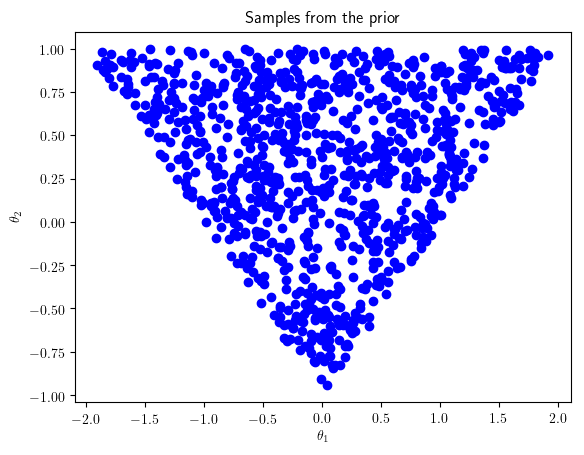
\includegraphics[width=0.48\textwidth]{./Thesis/images/chapter4/mae2_prior_samples.png}
    \end{center}
    \caption{Prior distribution proposed by Marin et al.\
      \cite{Marin2012}. The samples follow a triangular shape.}
  \label{fig:ma2_1}
\end{figure}

\noindent
The vector $\yb_0 = (y_1, \ldots, y_{100})$ used as the observation,
has been generated with $\thetab=(0.6, 0.2)$. The dimensionality of
the output $\yb$ is quite large, therefore we use summary
statistics. Considering that the ouptput vector represents a
time-series signal, we prefer the autocovariance as the summary
statistic; we incorporate the autocovariances with $lag=1$ and
$lag=2$, as shown in equation \eqref{eq:ma2_summary}. Hence, the
distance is defined as the squared euclidean distance between the
summary statistics.

\begin{gather} \label{eq:ma2_summary}
  s_1(\yb) = \frac{1}{T-1} \sum_{t=2}^T y_ty_{t-1}\\
  s_2(\yb) = \frac{1}{T-2} \sum_{t=3}^T y_ty_{t-2} \\
  s(\yb) = (s_1(\yb), s_2(\yb))\\
  d = ||s(\yb) - s(\yb_0)||_2^2
\end{gather}


\subsubsection*{Perform the inference}

As in the previous example, we perform the inference using the two
optimisation alternatives, the gradient-based and the Bayesian
optimisation. In this way, we compare the results obtained in each
step. For comparing the samples drawn with our implementation, we will
use the samples obtained with Rejection ABC. In figure \ref{fig:ma2_2}
we observe that in most cases the optimal distance $d_i^*$ is close to
zero in both optimisation approaches.

In figure \ref{fig:ma2_5}, we have chosen three different optimisation
examples for illustrating three different cases. In the first case,
both optimisation schemes lead to the creation of almost the same
bounding box. In the second case, the bounding box has a similar
shape, though different size and it is shifted along the $\theta_1$
axis. Finally, in the third case, the bounding boxes are completely
different. We can thus conclude that although fitting a surrogate
model has important computational advantages, there is no guarantee
that it will reproduce accurately the local region around the optimal
point. This approximation error may lead to the construction of a
considerably different proposal region, which in turn, explains the
differences in the histogram of the marginal distributions presented
in figure \ref{fig:ma2_3} and in the approximate posteriors in figure
\ref{fig:ma2_4}.

In figure \ref{fig:ma2_3}, we observe the histograms of the marginal
posteriors; undoubtedly, we observe that there is a significant
similarity between the three approaches. The Rejection ABC inference
has been set to infer 10000 accepted samples, with threshold
$\epsilon=0.1$. The large number of samples and the small distance
from the observations let treat them as ground-truth information. In
the table \ref{tab:ma2} we present the empirical mean $\mu$ and
standard deviation $\sigma$ for each inference approach. We observe
that there is a significant agreement between the approaches, which
verifies that the ROMC implementation provides sensible
results. Finally, in figure \ref{fig:ma2_4} we provide the ROMC
approximate posteriors using gradients and Bayesian optimisation; as
confirmed by the statistics in \ref{tab:ma2}, both posteriors have a
single mode, located at the same point, with a larger variance
observed in the Bayesian Optimisation case. The posteriors mode is
quite close to the parameter configuration that generated the data
i.e.\ $\thetab = (0.6, 0.2)$.

\begin{center} \label{tab:ma2}
\begin{tabular}{ c|c|c|c|c }
\hline
& $\mu_{\theta_1}$ & $\sigma_{\theta_1}$ & $\mu_{\theta_2}$ & $\sigma_{\theta_2}$ \\
\hline \hline
Rejection ABC & 0.516 & 0.142 & 0.07 & 0.172 \\
\hline
ROMC (gradient-based) & 0.495 & 0.136 & 0.048 & 0.178 \\
\hline
ROMC (Bayesian optimisation) & 0.510 & 0.156 & 0.108 & 0.183 \\
\hline
\end{tabular}
\end{center}

\begin{figure}[h]
    \begin{center}
      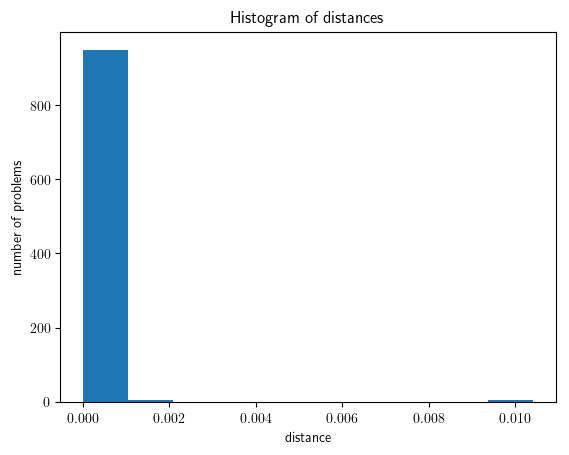
\includegraphics[width=0.48\textwidth]{./Thesis/images/chapter4/ma2_distance_hist.png}
      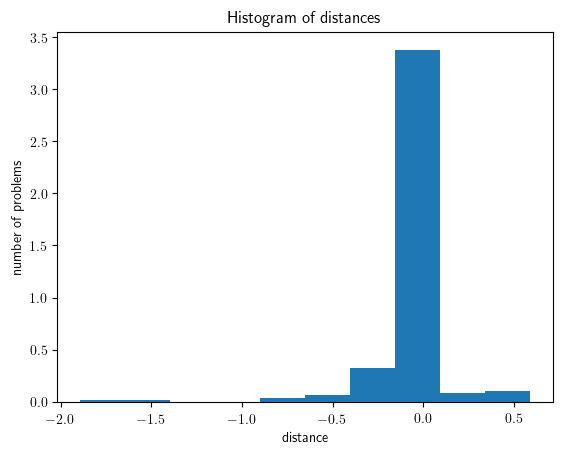
\includegraphics[width=0.48\textwidth]{./Thesis/images/chapter4/ma2_distance_hist_bo.png}
    \end{center}
  \caption{Histogram of distances $d_{i, i \in {1, \ldots, n_1}}^*$. The left graph corresponds to the gradient-based approach and the right one to the Bayesian optimisation approach.}
  \label{fig:ma2_2}
\end{figure}

\begin{figure}[h]
    \begin{center}
      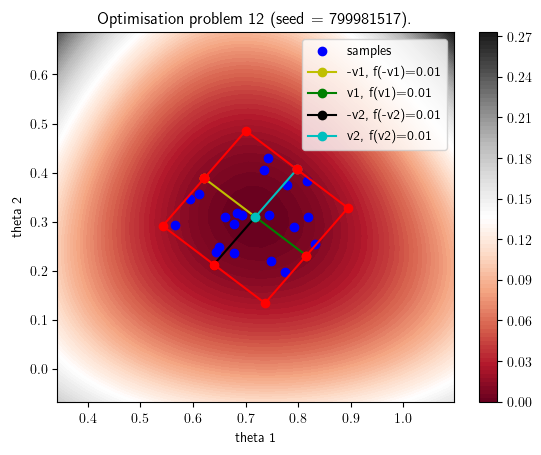
\includegraphics[width=0.48\textwidth]{./Thesis/images/chapter4/ma2_region_1.png}
      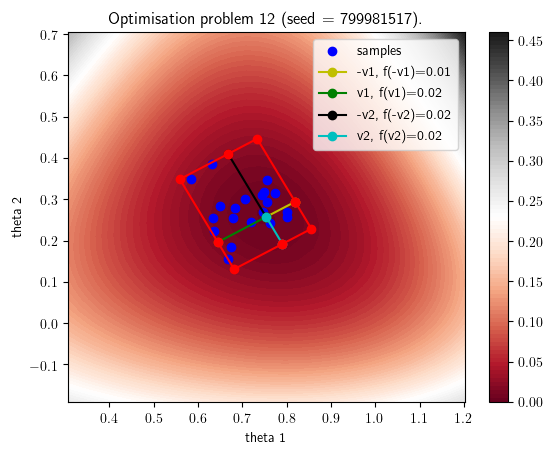
\includegraphics[width=0.48\textwidth]{./Thesis/images/chapter4/ma2_region_1_bo.png}\\
      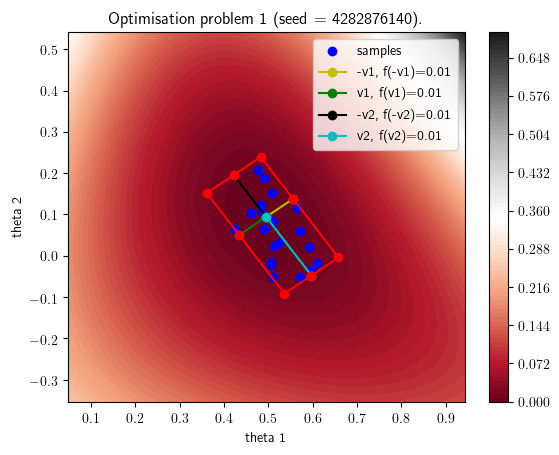
\includegraphics[width=0.48\textwidth]{./Thesis/images/chapter4/ma2_region_2.png}
      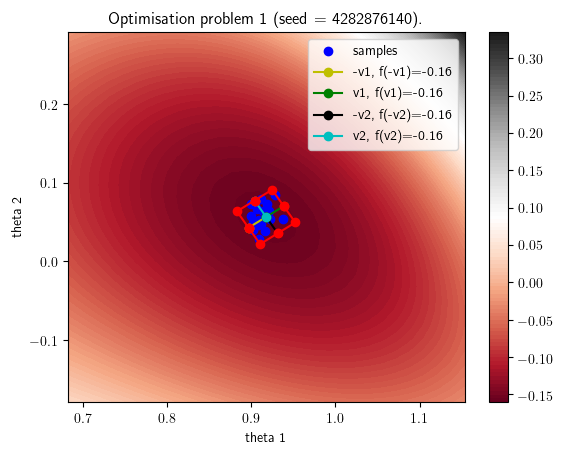
\includegraphics[width=0.48\textwidth]{./Thesis/images/chapter4/ma2_region_2_bo.png}\\
      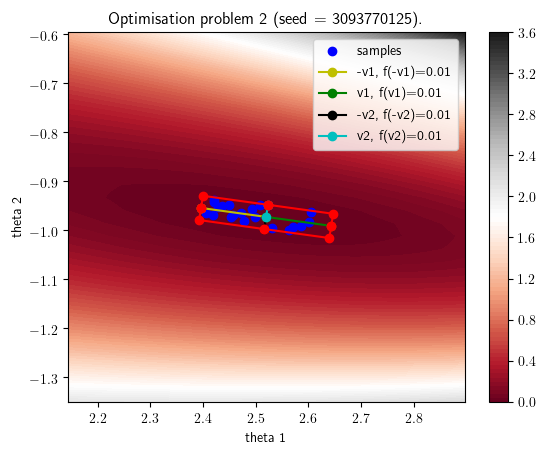
\includegraphics[width=0.48\textwidth]{./Thesis/images/chapter4/ma2_region_3.png}
      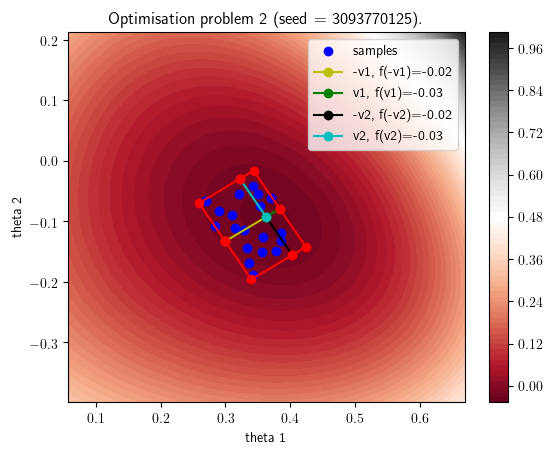
\includegraphics[width=0.48\textwidth]{./Thesis/images/chapter4/ma2_region_3_bo.png}
    \end{center}
  \caption{Visualisation of the acceptance region in 3 different optimisation problems. Each row illustrates a different optimisation problem, the left column corresponds to the gradient-based approach and the right column to the Bayesian optimisation approach. The examples have been chosen to illustrate three different cases; in the first case, both optimisation schemes lead to similar optimal point and bounding box, in the second case the bounding box is similar in shape but a little bit shifted to the right relatively to the gradient-based approach and in the third case, both the optimal point and the bounding box is completely different.}
  \label{fig:ma2_5}
\end{figure}


\begin{figure}[h]
    \begin{center}
      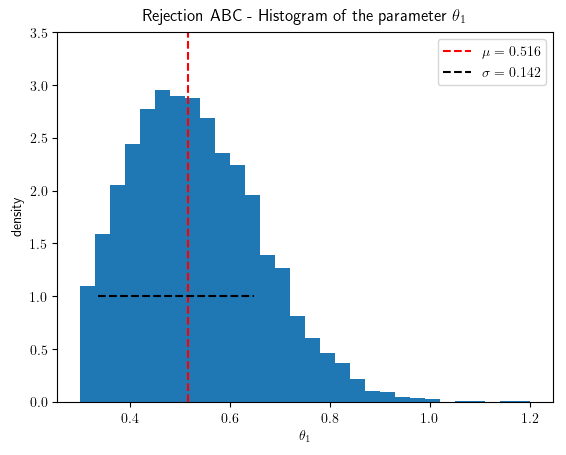
\includegraphics[width=0.48\textwidth]{./Thesis/images/chapter4/mae2_hist_t1_rejection.png}
      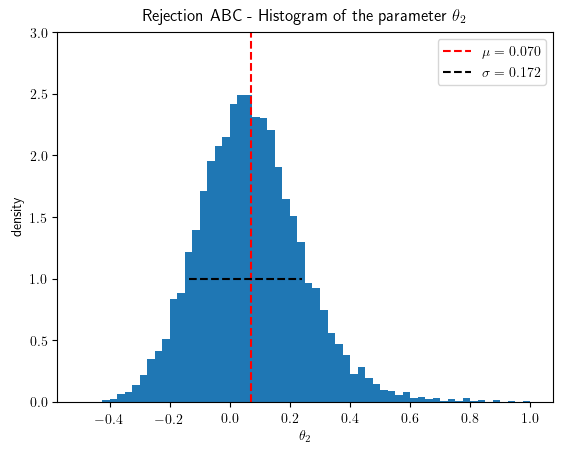
\includegraphics[width=0.48\textwidth]{./Thesis/images/chapter4/mae2_hist_t2_rejection.png}\\
      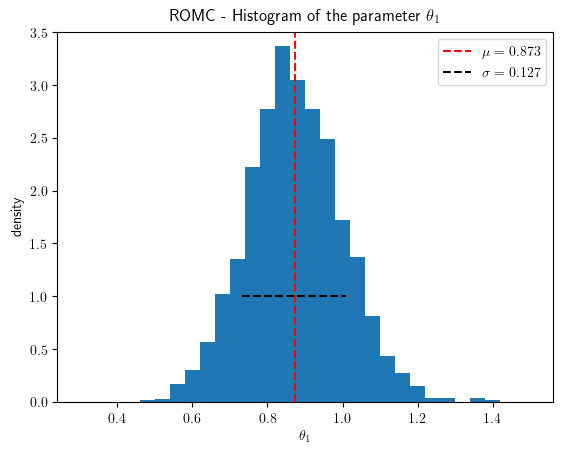
\includegraphics[width=0.48\textwidth]{./Thesis/images/chapter4/mae2_hist_t1_romc.png}
      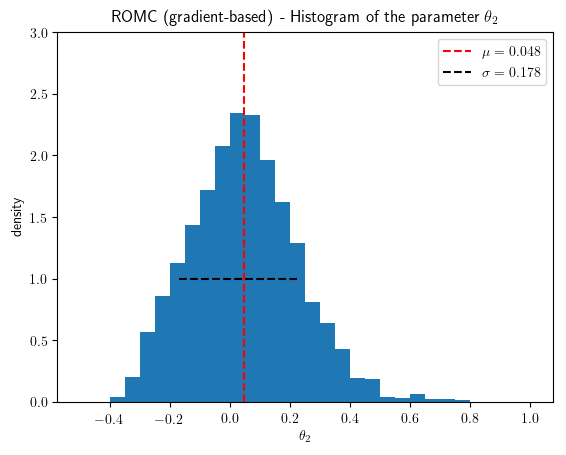
\includegraphics[width=0.48\textwidth]{./Thesis/images/chapter4/mae2_hist_t2_romc.png}\\
      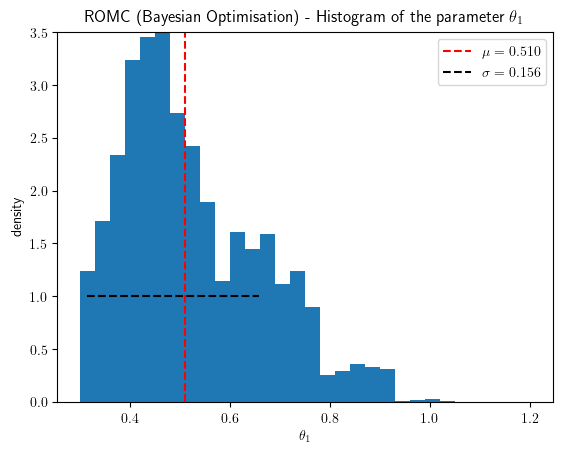
\includegraphics[width=0.48\textwidth]{./Thesis/images/chapter4/mae2_hist_t1_romc_bo.png}
      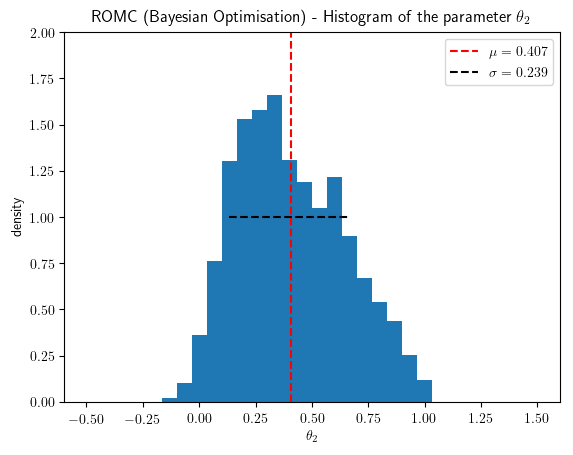
\includegraphics[width=0.48\textwidth]{./Thesis/images/chapter4/mae2_hist_t2_romc_bo.png}\\
    \end{center}
  \caption{Histogram of the marginal distribution for three different inference approaches; (a) in the first row, the approximate posterior samples are obtained using Rejection ABC sampling (b) in the second row, using ROMC sampling with gradient-based approach and (c) in the third row, using ROMC sampling with Bayesian optimisation approach. The vertical (red) line represents the samples mean $\mu$ and the horizontal (black) the standard deviation $\sigma$.}
  \label{fig:ma2_3}
\end{figure}


\begin{figure}[h]
    \begin{center}
      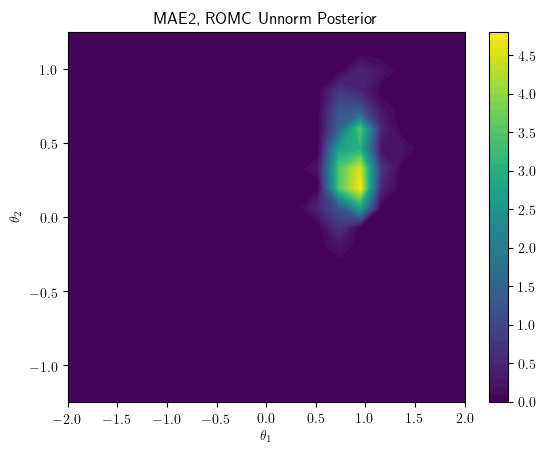
\includegraphics[width=0.48\textwidth]{./Thesis/images/chapter4/mae2_romc_posterior.png}
      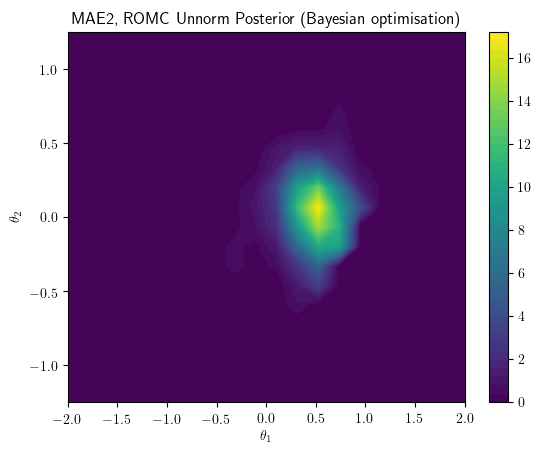
\includegraphics[width=0.48\textwidth]{./Thesis/images/chapter4/mae2_romc_posterior_bo.png}
    \end{center}
  \caption{ROMC approximate posteriors using gradient-based approach (left) and Bayesian optimisation approach (right).}
  \label{fig:ma2_4}
\end{figure}

